\documentclass[11pt,a4paper]{ctexart}
% Shared preamble for the assignment reports. Use with:
%   \documentclass[11pt,a4paper]{ctexart}  (XeLaTeX)
%   % Shared preamble for the assignment reports. Use with:
%   \documentclass[11pt,a4paper]{ctexart}  (XeLaTeX)
%   % Shared preamble for the assignment reports. Use with:
%   \documentclass[11pt,a4paper]{ctexart}  (XeLaTeX)
%   \input{../common/preamble.tex}
\usepackage[margin=2.3cm]{geometry}
\setmainfont{texgyretermes}[Extension=.otf,UprightFont=*-regular,BoldFont=*-bold,ItalicFont=*-italic,BoldItalicFont=*-bolditalic]
\setsansfont{texgyreheros}[Extension=.otf,UprightFont=*-regular,BoldFont=*-bold,ItalicFont=*-italic,BoldItalicFont=*-bolditalic]
\setmonofont{texgyrecursor}[Extension=.otf,UprightFont=*-regular,BoldFont=*-bold,ItalicFont=*-italic,BoldItalicFont=*-bolditalic]
\usepackage{amsmath,amssymb,mathtools,bm}
\usepackage{graphicx}
\usepackage{booktabs,multirow,makecell,array,tabularx}
\usepackage[table]{xcolor}
\usepackage[most]{tcolorbox}
\usepackage{enumitem}
\usepackage{listings}
\usepackage{subcaption}
\usepackage{siunitx}
\usepackage[hidelinks]{hyperref}
\usepackage[nameinlink,noabbrev]{cleveref}
\usepackage{float}

\setlength{\emergencystretch}{3em}
\linespread{1.15}
\setlist{leftmargin=*,itemsep=2pt,topsep=3pt}
\graphicspath{{figures/}}

\crefname{figure}{图}{图}
\crefname{table}{表}{表}
\crefname{section}{第}{第}
\creflabelformat{section}{#2#1#3 节}
\crefname{equation}{式}{式}
\crefformat{equation}{式~(#2#1#3)}

\lstset{basicstyle=\ttfamily\footnotesize,columns=fullflexible,breaklines=true,frame=single,
  framerule=0.3pt,rulecolor=\color{black!40},backgroundcolor=\color{black!3},
  keywordstyle=\color{blue!60!black}\bfseries,commentstyle=\color{green!40!black},
  numbers=left,numberstyle=\tiny\color{black!50},xleftmargin=1.5em}

% Interview boxes: question, model answer, common wrong answer.
\newtcolorbox{iqbox}[1]{enhanced,breakable,colback=blue!3,colframe=blue!45!black,boxrule=0.5pt,arc=1.5pt,
  left=4pt,right=4pt,top=3pt,bottom=3pt,fonttitle=\bfseries\small,title={面试追问：#1}}
\newtcolorbox{findingbox}[1][]{enhanced,breakable,colback=green!3,colframe=green!40!black,boxrule=0.5pt,arc=1.5pt,
  left=4pt,right=4pt,top=3pt,bottom=3pt,fonttitle=\bfseries\small,title={结论#1}}
\newtcolorbox{caveatbox}{enhanced,breakable,colback=orange!4,colframe=orange!60!black,boxrule=0.5pt,arc=1.5pt,
  left=4pt,right=4pt,top=3pt,bottom=3pt,fonttitle=\bfseries\small,title={不能推出的结论}}

\newcommand{\authorline}{ShaneLiu04\thanks{GitHub: \url{https://github.com/ShaneLiu04}。代码与原始指标见 edge-deploy 仓库各 lab 的 \texttt{artifacts/raw/}。本文基于公开课程材料独立完成，与课程团队无隶属关系。}}

\usepackage[margin=2.3cm]{geometry}
\setmainfont{texgyretermes}[Extension=.otf,UprightFont=*-regular,BoldFont=*-bold,ItalicFont=*-italic,BoldItalicFont=*-bolditalic]
\setsansfont{texgyreheros}[Extension=.otf,UprightFont=*-regular,BoldFont=*-bold,ItalicFont=*-italic,BoldItalicFont=*-bolditalic]
\setmonofont{texgyrecursor}[Extension=.otf,UprightFont=*-regular,BoldFont=*-bold,ItalicFont=*-italic,BoldItalicFont=*-bolditalic]
\usepackage{amsmath,amssymb,mathtools,bm}
\usepackage{graphicx}
\usepackage{booktabs,multirow,makecell,array,tabularx}
\usepackage[table]{xcolor}
\usepackage[most]{tcolorbox}
\usepackage{enumitem}
\usepackage{listings}
\usepackage{subcaption}
\usepackage{siunitx}
\usepackage[hidelinks]{hyperref}
\usepackage[nameinlink,noabbrev]{cleveref}
\usepackage{float}

\setlength{\emergencystretch}{3em}
\linespread{1.15}
\setlist{leftmargin=*,itemsep=2pt,topsep=3pt}
\graphicspath{{figures/}}

\crefname{figure}{图}{图}
\crefname{table}{表}{表}
\crefname{section}{第}{第}
\creflabelformat{section}{#2#1#3 节}
\crefname{equation}{式}{式}
\crefformat{equation}{式~(#2#1#3)}

\lstset{basicstyle=\ttfamily\footnotesize,columns=fullflexible,breaklines=true,frame=single,
  framerule=0.3pt,rulecolor=\color{black!40},backgroundcolor=\color{black!3},
  keywordstyle=\color{blue!60!black}\bfseries,commentstyle=\color{green!40!black},
  numbers=left,numberstyle=\tiny\color{black!50},xleftmargin=1.5em}

% Interview boxes: question, model answer, common wrong answer.
\newtcolorbox{iqbox}[1]{enhanced,breakable,colback=blue!3,colframe=blue!45!black,boxrule=0.5pt,arc=1.5pt,
  left=4pt,right=4pt,top=3pt,bottom=3pt,fonttitle=\bfseries\small,title={面试追问：#1}}
\newtcolorbox{findingbox}[1][]{enhanced,breakable,colback=green!3,colframe=green!40!black,boxrule=0.5pt,arc=1.5pt,
  left=4pt,right=4pt,top=3pt,bottom=3pt,fonttitle=\bfseries\small,title={结论#1}}
\newtcolorbox{caveatbox}{enhanced,breakable,colback=orange!4,colframe=orange!60!black,boxrule=0.5pt,arc=1.5pt,
  left=4pt,right=4pt,top=3pt,bottom=3pt,fonttitle=\bfseries\small,title={不能推出的结论}}

\newcommand{\authorline}{ShaneLiu04\thanks{GitHub: \url{https://github.com/ShaneLiu04}。代码与原始指标见 edge-deploy 仓库各 lab 的 \texttt{artifacts/raw/}。本文基于公开课程材料独立完成，与课程团队无隶属关系。}}

\usepackage[margin=2.3cm]{geometry}
\setmainfont{texgyretermes}[Extension=.otf,UprightFont=*-regular,BoldFont=*-bold,ItalicFont=*-italic,BoldItalicFont=*-bolditalic]
\setsansfont{texgyreheros}[Extension=.otf,UprightFont=*-regular,BoldFont=*-bold,ItalicFont=*-italic,BoldItalicFont=*-bolditalic]
\setmonofont{texgyrecursor}[Extension=.otf,UprightFont=*-regular,BoldFont=*-bold,ItalicFont=*-italic,BoldItalicFont=*-bolditalic]
\usepackage{amsmath,amssymb,mathtools,bm}
\usepackage{graphicx}
\usepackage{booktabs,multirow,makecell,array,tabularx}
\usepackage[table]{xcolor}
\usepackage[most]{tcolorbox}
\usepackage{enumitem}
\usepackage{listings}
\usepackage{subcaption}
\usepackage{siunitx}
\usepackage[hidelinks]{hyperref}
\usepackage[nameinlink,noabbrev]{cleveref}
\usepackage{float}

\setlength{\emergencystretch}{3em}
\linespread{1.15}
\setlist{leftmargin=*,itemsep=2pt,topsep=3pt}
\graphicspath{{figures/}}

\crefname{figure}{图}{图}
\crefname{table}{表}{表}
\crefname{section}{第}{第}
\creflabelformat{section}{#2#1#3 节}
\crefname{equation}{式}{式}
\crefformat{equation}{式~(#2#1#3)}

\lstset{basicstyle=\ttfamily\footnotesize,columns=fullflexible,breaklines=true,frame=single,
  framerule=0.3pt,rulecolor=\color{black!40},backgroundcolor=\color{black!3},
  keywordstyle=\color{blue!60!black}\bfseries,commentstyle=\color{green!40!black},
  numbers=left,numberstyle=\tiny\color{black!50},xleftmargin=1.5em}

% Interview boxes: question, model answer, common wrong answer.
\newtcolorbox{iqbox}[1]{enhanced,breakable,colback=blue!3,colframe=blue!45!black,boxrule=0.5pt,arc=1.5pt,
  left=4pt,right=4pt,top=3pt,bottom=3pt,fonttitle=\bfseries\small,title={面试追问：#1}}
\newtcolorbox{findingbox}[1][]{enhanced,breakable,colback=green!3,colframe=green!40!black,boxrule=0.5pt,arc=1.5pt,
  left=4pt,right=4pt,top=3pt,bottom=3pt,fonttitle=\bfseries\small,title={结论#1}}
\newtcolorbox{caveatbox}{enhanced,breakable,colback=orange!4,colframe=orange!60!black,boxrule=0.5pt,arc=1.5pt,
  left=4pt,right=4pt,top=3pt,bottom=3pt,fonttitle=\bfseries\small,title={不能推出的结论}}

\newcommand{\authorline}{ShaneLiu04\thanks{GitHub: \url{https://github.com/ShaneLiu04}。代码与原始指标见 edge-deploy 仓库各 lab 的 \texttt{artifacts/raw/}。本文基于公开课程材料独立完成，与课程团队无隶属关系。}}

\graphicspath{{../../solutions/edge-runtime/runtime-compare/artifacts/figures/}}

\title{同一张网，六条 CPU 推理路径：\\PyTorch、ONNX Runtime fp32 / int8、LiteRT、ExecuTorch 与 TVM}
\author{\authorline}
\date{2026 年 11 月}

\begin{document}
\maketitle

\begin{abstract}
本仓库 lab2 训练的 micronet（MicroMobileNetV2~\cite{mobilenetv2} 的缩小版，CIFAR-10，BN 折叠后的 fp32）原样交给 6 条推理路径：
PyTorch eager、ONNX Runtime~\cite{ort} fp32、ONNX Runtime int8（lab2 部署用的 QDQ + MinMax 校准~\cite{jacob2018}）、
LiteRT~\cite{litert}、ExecuTorch~\cite{executorch}（XNNPACK~\cite{xnnpack} 委托）和 Apache TVM~\cite{tvm} 的 Relax~\cite{relax} + LLVM（不调优）。
每条路径 1 个线程，跑完整个测试集（10,000 张，batch 1），比较精度、与 PyTorch 的逐图一致性和每张图的 CPU 时间。
平台是 AutoDL 的无卡容器：看得见 2 × Xeon Platinum 8470Q 的 208 个逻辑核，cgroup 只给 0.5 核、2 GB 内存，所以时间一律用进程 CPU 时间，每条路径 3 个新进程取中位数。

主要结论：
（a）四个 fp32 运行时与 PyTorch 逐图同答：top-1 都是 88.16\%，10,000 张图 argmax 全部相同，最大 logit 差 $5.7\times10^{-6}$；
（b）ORT int8 是唯一掉点的路径，也是最快的：88.09\%（与 lab2 发布的数相同），与 fp32 逐图一致 99.05\%，每张图 127~$\mu$s，是 ORT fp32 的 1/1.60，模型文件是 1/2.59；
（c）三个部署运行时的排序在同一批 3 个进程内互不重叠、下午三批运行中也不变：LiteRT 166~$\mu$s $<$ ExecuTorch 192 $<$ ORT fp32 202；
（d）PyTorch eager 1173~$\mu$s，是 ORT fp32 的 5.8 倍；不调优的 TVM 4107~$\mu$s，是 PyTorch 的 3.5 倍。在 0.5 核上 MetaSchedule~\cite{metaschedule} 调不完这张网。
为了在 2 GB 里把 6 行跑通，本报告记录了 8 个环境问题及其处理，其中 apache-tvm-ffi 0.1.15 / 0.1.16 序列化即段错误、TVM 只要能导入 torch 就现编 C++ 扩展两条，
直接决定了 TVM 那一行能不能出数。
\end{abstract}

\tableofcontents
\newpage

\section{这个实验要回答什么}

\subsection{课程背景}
MLC（Machine Learning Compilation）课程~\cite{mlc} 的作业 1 把一个小 CNN 从 PyTorch 迁进 TVM 的 IRModule，把一部分算子换成外部库，再对卷积做调度变换；
作业 2--4 写 TensorIR、跑自动调优、把结果接回编译流程。它们问的是同一个问题：同一张图，交给不同的执行引擎，结果是否一样、快慢差多少、差在哪里。
本仓库此前把这个问题拆开回答过：lab2 用 ORT 跑导出的 ONNX，int8-kernels 用 ORT 的 \texttt{QLinearConv} 做逐位参照，tensor-program-tuning 自己写搜索器调矩阵乘。
缺的是一张“同一份权重、几套生产运行时”的端到端表，这正是本实验补上的。

\subsection{要回答的三个问题}
\begin{enumerate}
  \item 转换是否保真？五个运行时各自走自己的导出链（ONNX、litert-torch、\texttt{torch.export} + XNNPACK 分区、Relax ONNX 前端），10,000 张图上和 PyTorch 是否同答。
  \item 单线程 CPU 上谁快、快多少？在一张很小的网上，框架派发开销、算子库和编译器默认调度各占多少。
  \item int8 在这台 Sapphire Rapids 上能带来多少？和 lab2 在 Ice Lake 虚拟机上的 1.47 倍是什么关系。
\end{enumerate}

\subsection{和原课程的差异}
作业 1 在 TVM 内部完成迁移与替换；这里不安装 \texttt{mlc-ai}，改成让 5 个生产运行时各跑同一份权重，TVM 只占其中一行。
作业 2--4 的调优在这台机器上做不了（\cref{sec:pitfalls} 第 8 条），对应内容在 tensor-program-tuning。无卡模式没有 CUDA 设备，因此没有 GPU 委托这一条线。

\section{设置}\label{sec:method}

\subsection{模型与数据}
模型是 lab2 发布的 checkpoint（\texttt{micronet.pt}），经 lab2 的 \texttt{fold\_model} 把 BN 折进卷积后以 fp32 导出；输入 $1\times3\times32\times32$，输出 10 类 logits。
测试集是 CIFAR-10 的 10,000 张，按 lab2 的均值方差归一化。int8 校准用训练集按种子 0 打乱后的前 512 张。

\subsection{六条路径}
\begin{table}[H]
\centering\small
\caption{六条路径与各自的导出链。版本取自 \texttt{summary.json} 每行的 \texttt{version} / \texttt{torch} 字段}\label{tab:paths}
\begin{tabularx}{\linewidth}{>{\raggedright\arraybackslash}p{1.8cm}>{\raggedright\arraybackslash}p{2.6cm}>{\raggedright\arraybackslash}X>{\raggedright\arraybackslash}X}
\toprule
路径 & 版本 & 导出 & 执行 \\
\midrule
PyTorch & torch 2.8.0 & 无 & \texttt{inference\_mode}，1 线程 \\
ORT fp32 & onnxruntime 1.31.1 & \texttt{torch.onnx.export}，opset 17，静态 batch 1 & CPU EP，intra / inter 线程各 1 \\
ORT int8 & onnxruntime 1.31.1 & 动态 batch 导出，\texttt{quant\_pre\_process}，\texttt{quantize\_static} & QDQ，权重逐通道 int8、激活 uint8、MinMax；CPU EP 1 线程 \\
LiteRT & ai-edge-litert 2.3.0 & litert-torch 0.10.0（torch 2.14.1+cpu） & \texttt{Interpreter}，1 线程 \\
ExecuTorch & executorch 1.6.0 & \texttt{torch.export}，再 \texttt{to\_edge\_\allowbreak transform\_\allowbreak and\_lower}（XNNPACK 分区）；torch 2.15.0+cpu & \texttt{Runtime}，线程池重置为 1 \\
TVM & apache-tvm 0.27.0.post1 & Relax ONNX 前端读 ORT fp32 那份 ONNX & \texttt{tvm.compile}，LLVM，\texttt{mcpu} 为 sapphirerapids，1 核；Relax VM \\
\bottomrule
\end{tabularx}
\end{table}

\subsection{平台与计时}
AutoDL 无卡容器，Python 3.12。\texttt{/sys/fs/cgroup/cpu.max} 是 \texttt{50000 100000}，即每 100~ms 只能跑 50~ms；\texttt{memory.max} 是 2,147,483,648 字节。
在这样的配额下，墙钟时间主要量的是配额：一段 2 秒的 Python 自增循环，本地 4 核 Ice Lake 虚拟机跑 12,542,873 次，这里只有 9,850,970 次。
因此所有时间都用 \texttt{time.process\_time()}，它只计入进程真正占用 CPU 的时间。

每条路径在一个独立的子进程里：先构建（导出、转换、量化或编译），用第一张图核对输出形状，再做两种计时：
\begin{itemize}
  \item \texttt{cpu\_us\_eval}：按 batch 1 跑完 10,000 张测试图，总 CPU 时间除以 10,000。这是报告的主口径，它同时给出精度和逐图 logits。
  \item \texttt{cpu\_us}：同一张图预热 20 次后重复 200 次的平均 CPU 时间。
\end{itemize}
每条路径用 3 个新进程各跑一遍（\texttt{part-<路径>-t<轮>.json}），汇总时取中位数，并保留最小值与最大值（\texttt{rtcmp.measure.combine}）。
精度和 logits 是确定的，取自第 1 轮。一致性指标是和 PyTorch 那一轮保存的 logits 比：最大绝对差，以及 argmax 相同的图所占比例。

\section{结果}\label{sec:results}

\begin{figure}[H]
\centering
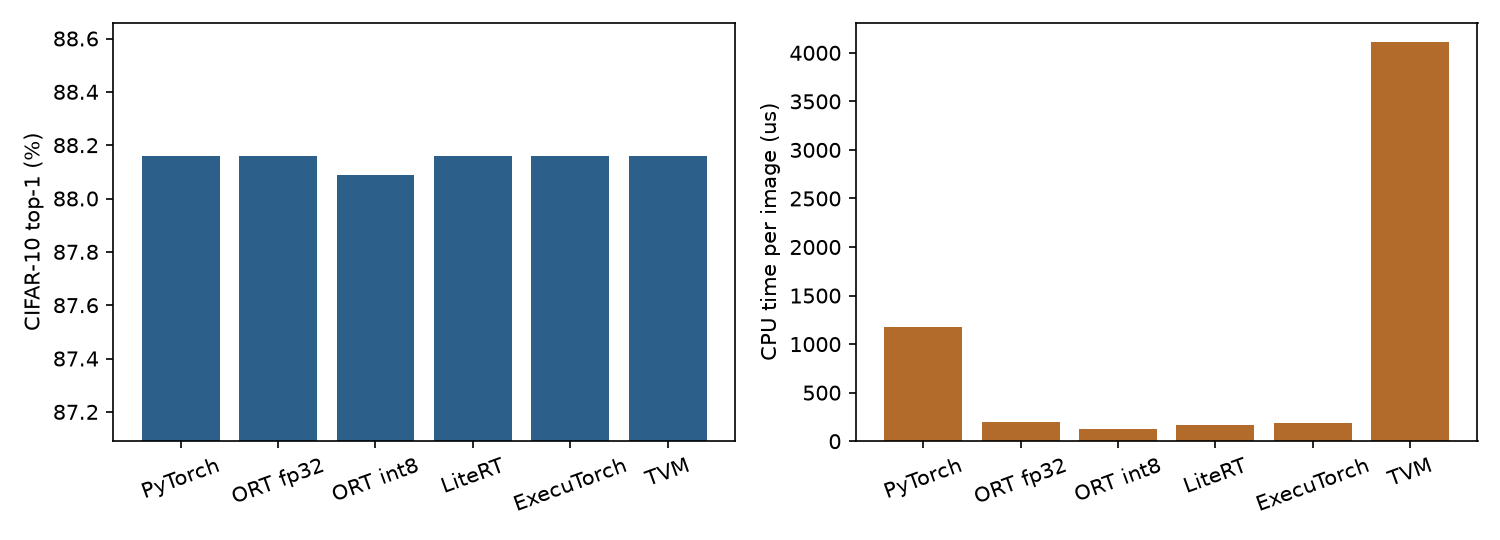
\includegraphics[width=\linewidth]{runtime_compare.png}
\caption{六条路径的 top-1（左）与每张图的 CPU 时间（右，\texttt{cpu\_us\_eval}，3 个进程的中位数）。}\label{fig:main}
\end{figure}

\begin{table}[H]
\centering\small
\caption{完整结果（\texttt{summary.json}）。CPU 时间括号里是 3 个进程的最小--最大；RSS 是整个子进程的峰值，含加载数据与 PyTorch 模型}\label{tab:main}
\setlength{\tabcolsep}{3.5pt}
\begin{tabular}{lrrrrrr}
\toprule
路径 & top-1 & argmax 一致 & 最大 logit 差 & CPU 时间 / 图 ($\mu$s) & 模型文件 (B) & 峰值 RSS (MB) \\
\midrule
PyTorch eager & 88.16\% & 1 & 0 & 1173（1144--1224） & — & 660 \\
ORT fp32 & 88.16\% & 1 & $5.7\times10^{-6}$ & 202（201--213） & 843,513 & 709 \\
ORT int8 & 88.09\% & 0.9905 & 1.74 & 127（125--134） & 326,171 & 997 \\
LiteRT & 88.16\% & 1 & $5.7\times10^{-6}$ & 166（161--175） & 855,844 & 914 \\
ExecuTorch & 88.16\% & 1 & $5.7\times10^{-6}$ & 192（185--195） & 843,816 & 626 \\
TVM（不调优） & 88.16\% & 1 & $5.7\times10^{-6}$ & 4107（3979--4217） & — & 563 \\
\bottomrule
\end{tabular}
\end{table}

\subsection{转换保真}
四个 fp32 运行时走的是四条互不相同的导出链，结果却完全一致：最大 logit 差都是 $5.7220\times10^{-6}$（float32 在 logit 量级上的几个 ulp），10,000 张图的 argmax 和 PyTorch 全同。
这说明 BN 折叠之后这张网里没有哪个算子在转换时被近似或改写成不等价的形式；后面的时间差别都来自执行方式，不来自算的东西不同。

int8 的最大 logit 差 1.74 是量化误差本身，不是转换错误。要看的是两件事：top-1 88.09\% 只比 fp32 低 0.07 个点，与 lab2 发布的结果相同；
和 fp32 逐图一致 99.05\%，也就是 95 张图换了答案，其中错改对与对改错相抵后净少 7 张。

\subsection{时间：三档}
\Cref{fig:main} 的右图分成三档。第一档是三个部署运行时与 int8：127--202~$\mu$s。第二档是 PyTorch eager：1173~$\mu$s，是 ORT fp32 的 5.80 倍。第三档是不调优的 TVM：4107~$\mu$s。

\paragraph{第一档内部。} LiteRT 166、ExecuTorch 192、ORT fp32 202。三者的 3 个进程范围（161--175、185--195、201--213）互不重叠；
同一天下午的三批运行中排序都相同。
三者都把卷积交给手写的 SIMD 内核（LiteRT 默认走 XNNPACK，ExecuTorch 显式委托 XNNPACK，ORT 用 MLAS），差距在 20\% 以内，来自图级融合和调用开销的不同；本实验没有拆分这一部分。

\paragraph{int8。} ORT int8 比 ORT fp32 少 1.60 倍 CPU 时间、模型小 2.59 倍。lab2 在 Ice Lake 虚拟机上测的是 1.47 倍（372.4 → 253.9~$\mu$s，1 线程墙钟）。
两个数方向一致，但机器（Ice Lake 对 Sapphire Rapids）、时钟（墙钟对 CPU 时间）都不同，不能放进同一张表比较大小。

\paragraph{PyTorch eager。} micronet 每层的计算量很小（输入只有 $32\times32$），eager 模式每个算子都要经过 Python 调用、调度器派发和张量分配，这部分开销是常数，不随计算量缩小。
推断它占了 1173~$\mu$s 中的大部分；输入变大时，这个 5.8 倍会向 1 靠近。本实验只测了 $32\times32$，这一条没有验证。

\paragraph{TVM。} 4107~$\mu$s，比 PyTorch 还慢 3.5 倍，但和 PyTorch 逐图同答。\texttt{tvm.compile} 的默认流程把 Relax 图降成 TensorIR 后直接交给 LLVM，
没有给 CPU 上的 conv2d 做分块、向量化之类的调度；补这一步正是 MLC 作业 2--4 与 MetaSchedule 的内容。这一行量出的是“编译器不调度”的代价，不是 TVM 的上限。

\subsection{两种计时口径}
\begin{figure}[H]
\centering
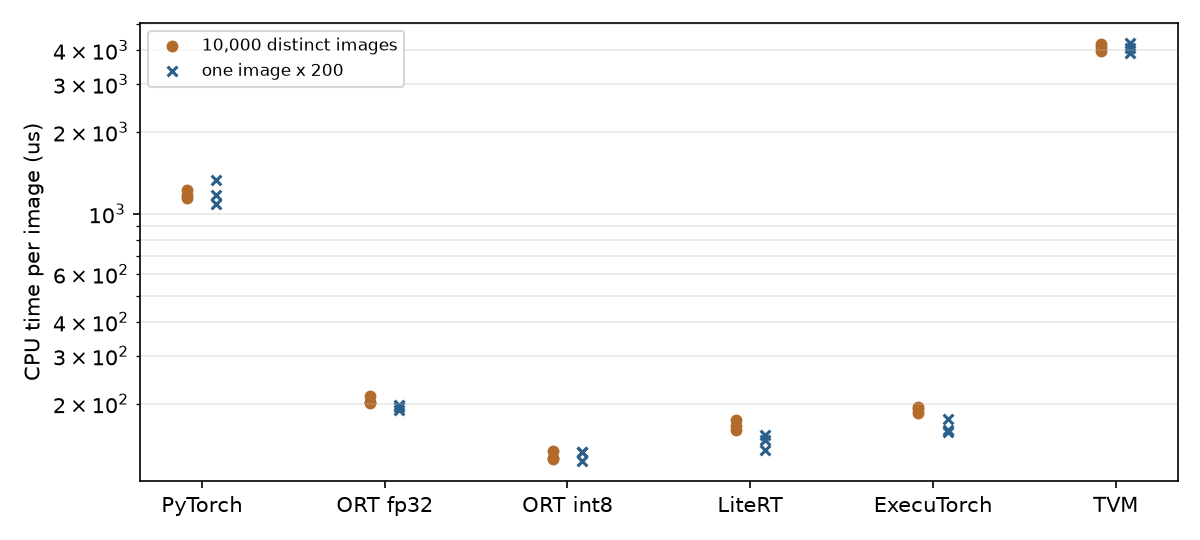
\includegraphics[width=0.9\linewidth]{runtime_trials.png}
\caption{每个进程的两种 CPU 时间（对数纵轴）。圆点：10,000 张不同图的平均；叉：同一张图重复 200 次。每条路径 3 个进程。}\label{fig:trials}
\end{figure}

同一张图重复 200 次（\texttt{cpu\_us}）多数时候更快：LiteRT 148 对 166、ExecuTorch 160 对 192，因为输入一直在缓存里，也省掉了换输入时的张量构造。ORT int8 反而慢 5\%（133 对 127）。
两种口径给出的排序相同（\cref{fig:trials}）。报告以 \texttt{cpu\_us\_eval} 为准：它的样本量是 10,000，且输入在变，更接近部署时的情形。

\begin{findingbox}[：三句话]
\begin{enumerate}
  \item 四条 fp32 导出链与 PyTorch 逐图同答（最大 logit 差 $5.7\times10^{-6}$），时间差别全部来自执行方式。
  \item 单线程 CPU 上，int8（127~$\mu$s）$<$ LiteRT（166）$<$ ExecuTorch（192）$<$ ORT fp32（202）$\ll$ PyTorch eager（1173）$\ll$ 不调优的 TVM（4107）。
  \item 在这张小网上，框架派发与编译器调度各自的代价都比算子库之间的差别大一个数量级。
\end{enumerate}
\end{findingbox}

\section{在 0.5 核、2 GB 里把 6 行跑通}\label{sec:pitfalls}

{\sloppy 下面 8 条是这次运行中实际遇到的问题，每条在脚本里都有对应的处理（\texttt{scripts/run\_autodl.sh}）。\par}

\begin{enumerate}\sloppy
  \item \textbf{墙钟量的是配额}（\cref{sec:method}）。对比只用 CPU 时间。
  \item \textbf{页缓存算在 2 GB 里。} 一次带 TVM 调优的完整运行中，调优进程被杀之后，第 3 轮的 ORT fp32、ORT int8、LiteRT、ExecuTorch 都以 SIGKILL 退出，而 \texttt{memory.events} 的 \texttt{oom\_kill} 一直是 0。
        那次运行结束、没有任何实验进程时，cgroup 仍记着 1.48 GB，其中匿名内存 321 MB、页缓存 1059 MB。
        \texttt{/proc/sys/vm/drop\_caches} 与 \texttt{memory.reclaim} 都不可写（5.15 内核也没有后者），\texttt{evict\_page\_cache.py} 对每个文件调 \texttt{posix\_fadvise(DONTNEED)}，一次把 cgroup 从 1486 MiB 降到 551 MiB。
        最终运行在每个子进程前回收一次，18 个进程全部成功。谁发出的 SIGKILL 无法确认，能确认的只是回收之后不再发生。
  \item \textbf{ORT 的校准器按物理核数开线程。} \texttt{quantize\_static} 内部创建的会话不受调用方线程设置约束，进程里有 105 个线程；batch 1 校准 7 分钟用掉 3.5 分钟 CPU 仍未完成。
        改成 lab2 的做法（动态 batch，每批 64 张），并在量化期间把 \texttt{InferenceSession} 包一层、强制 1 线程，本地冒烟测试 1.6~s CPU 时间完成。
  \item \textbf{TVM 只要能导入 torch，就现编一个 C++ 扩展。} \texttt{tvm/relax/base\_py\_module.py} 无条件调用 \texttt{load\_torch\_c\_dlpack\_extension()}，环境变量 \texttt{TVM\_FFI\_DISABLE\_TORCH\_C\_DLPACK} 只管 \texttt{tvm\_ffi} 自己那一处。
        编译时 TVM 进程 700 MB、构建用的 Python 530 MB、\texttt{cc1plus} 620 MB，合计超过 2 GB，\texttt{import tvm} 以 137 退出。
        TVM 这一行不需要 torch：专用的 \texttt{tvmvenv} 里放一个 \texttt{sitecustomize.py}，设 \texttt{sys.modules["torch"] = None}，导入后峰值 RSS 207 MB。
  \item \textbf{apache-tvm-ffi 0.1.15 与 0.1.16 搭配 TVM 0.27.0.post1 时，任何 \texttt{save\_json} 都段错误}（\texttt{tvm::ffi::ToJSONGraph}），连一个 \texttt{IntImm} 也一样；0.1.14 与 0.1.14.post0 正常。
        TVM 的元数据只写 \texttt{apache-tvm-ffi>=0.1.14.post0}，pip 默认装最新版。只编译不序列化时 0.1.16 也能得到同样的精度，所以这个问题在调优写数据库时才暴露。
  \item \textbf{TVM 0.27 不再接受字符串目标。} \texttt{"llvm -mcpu=sapphirerapids -num-cores 1"} 报错，要写成 \texttt{\{"kind": "llvm", "mcpu": "sapphirerapids", "num-cores": 1\}}。
  \item \textbf{torch 版本要求互斥。} executorch 1.6 钉死 \texttt{torch==2.15.0}，litert-torch 0.10 要求 \texttt{torch<2.15}；PyPI 上的 torch 2.15 是 CUDA 13 轮子，无卡模式缺 \texttt{libcudart.so.13} 与 nvshmem。
        两个 torch 都从 PyTorch 的 CPU 索引装，分进两个虚拟环境；计时脚本每条路径一个子进程，用 \texttt{RTCMP\_PY\_<NAME>} 指定各自的解释器。
  \item \textbf{MetaSchedule 在 0.5 核上调不完。} micronet 拆出 24 个调优任务。builder 默认按逻辑核数（208）开进程池，改成 1 后，调度器给第一个任务的第一批 62 个候选，15 分钟到超时时 runner 仍未量完。
        按每个任务 32 次试验算，全网要 768 次，本机上要数小时，所以表里只有不调优的 TVM。
\end{enumerate}

\begin{iqbox}{为什么不直接用墙钟时间，再除以 0.5？}
配额按 100~ms 一个周期发放：进程在一个周期里跑满 50~ms 后被挂起到下一个周期。单次推理只有几百微秒，大多数调用落在“跑”的那一段，和独占核一样快；
碰上挂起的那一次要多等几十毫秒。所以墙钟的平均值取决于这几次挂起落在哪里，除以 0.5 得不到工作量。
同一张图重复 200 次时，ORT fp32 三个进程的墙钟平均是 189--358~$\mu$s，同一批调用的 CPU 时间是 189--198~$\mu$s。
\end{iqbox}

\begin{iqbox}{四个 fp32 运行时为什么能逐图同答，而不是“差不多”？}
它们都用 fp32 累加，同一层的乘加顺序可能不同，但 float32 的舍入误差在 logit 上只有 $10^{-6}$ 量级；argmax 只有在前两名 logit 相差小于这个量级时才会翻转，10,000 张图里没有这样的图。
int8 不同：每层输出都被量化到 256 个级别，误差是 $10^{-1}$--$1$ 量级，所以有 95 张图翻转。
\end{iqbox}

\section{和 mlsys-infra 的关系}
姊妹仓库 mlsys-infra 的 M10（ML 编译器）讨论的是 GPU 上的图级融合与 kernel 生成，这里的第二档、第三档是同一件事在 CPU 小网上的表现：
eager 的派发开销对应 GPU 上的 kernel launch 开销，CUDA graph 解决的问题在这里由“提前导出成静态图”解决；不调优的 TVM 慢，对应 GPU 上没有 Triton 自动调优的 kernel。
int8 这一行与 mlsys-infra M17 的 LLM.int8 / W8A8 讨论的是同一种量化格式，但这里是激活也量化的静态 QDQ，没有离群值通道的特殊处理。

\section{不能推出的结论}\label{sec:caveat}

\begin{caveatbox}
\begin{itemize}
  \item 不能推出这台 8470Q 空闲时的延迟。0.5 核配额下 CPU 时间接近单线程工作量，但频率与缓存和独占核不同；同一天中午第一次运行里 ORT fp32 重复 20 次是 307~$\mu$s，下午 8 个进程的 \texttt{cpu\_us\_eval} 在 201--244~$\mu$s。同一批内部的排序可靠，跨批的绝对值能差一半。
  \item 不能和 lab2 的 1.47 倍比大小：机器、时钟都不同（\cref{sec:results}）。
  \item 不能推出 TVM 慢。4107~$\mu$s 是不调优的结果；调优能降到多少，这台机器回答不了。
  \item 不能推出 PyTorch eager 在大网络上也慢 5.8 倍。派发开销占比随输入增大而下降，本实验只测了 $32\times32$。
  \item 不能推出 LiteRT / ExecuTorch / ORT 在多线程或 ARM 上的排序。本实验只有 x86、1 线程、fp32（外加 ORT int8）；LiteRT 与 ExecuTorch 的 int8 路径没有跑。
  \item 峰值 RSS 包含加载 CIFAR-10 与 PyTorch 模型的开销，不是运行时本身的内存占用；ORT int8 那一行还包括校准。
\end{itemize}
\end{caveatbox}

\section{复现}

\begin{lstlisting}[language=bash,numbers=none]
# repo root, Linux; needs lab2's checkpoints/micronet.pt and .data/cifar10.npz
python -m pytest -q solutions/edge-runtime/runtime-compare/tests      # 5 tests
bash solutions/edge-runtime/runtime-compare/scripts/run_autodl.sh     # 6 paths x 3 processes, three venvs
python solutions/edge-runtime/runtime-compare/scripts/run_experiments.py --plot   # redraw figures from raw files
# outputs
#   artifacts/raw/part-<path>-t<k>.json  summary.json  runs.jsonl
#   artifacts/figures/runtime_compare.png  runtime_trials.png
\end{lstlisting}

{\sloppy \texttt{run\_autodl.sh} 开头写了三个虚拟环境各装什么。模型文件与参考 logits 写在 \texttt{artifacts/work/}（不入库）。
\texttt{claims.json} 里 18 条 \texttt{rt-*} 对 \texttt{summary.json} 做数值校验。\par}

\begin{thebibliography}{99}
\bibitem{mobilenetv2} M.~Sandler, A.~Howard, M.~Zhu, A.~Zhmoginov, L.-C.~Chen. MobileNetV2: Inverted Residuals and Linear Bottlenecks. \emph{CVPR}, 2018.
\bibitem{ort} ONNX Runtime developers. ONNX Runtime. \url{https://onnxruntime.ai}, 2021.
\bibitem{jacob2018} B.~Jacob, S.~Kligys, B.~Chen, M.~Zhu, M.~Tang, A.~Howard, H.~Adam, D.~Kalenichenko. Quantization and Training of Neural Networks for Efficient Integer-Arithmetic-Only Inference. \emph{CVPR}, 2018.
\bibitem{litert} Google AI Edge. LiteRT (formerly TensorFlow Lite). \url{https://ai.google.dev/edge/litert}, 2024.
\bibitem{executorch} PyTorch team. ExecuTorch: on-device AI across mobile, embedded and edge for PyTorch. \url{https://github.com/pytorch/executorch}, 2023.
\bibitem{xnnpack} Google. XNNPACK: High-efficiency floating-point neural network inference operators. \url{https://github.com/google/XNNPACK}, 2019.
\bibitem{tvm} T.~Chen, T.~Moreau, Z.~Jiang, L.~Zheng, E.~Yan, M.~Cowan, H.~Shen, L.~Wang, Y.~Hu, L.~Ceze, C.~Guestrin, A.~Krishnamurthy. TVM: An Automated End-to-End Optimizing Compiler for Deep Learning. \emph{OSDI}, 2018.
\bibitem{relax} R.~Lai, J.~Shao, S.~Feng, et~al. Relax: Composable Abstractions for End-to-End Dynamic Machine Learning. arXiv:2311.02103, 2023.
\bibitem{metaschedule} J.~Shao, X.~Zhou, S.~Feng, B.~Hou, R.~Lai, H.~Jin, W.~Lin, M.~Masuda, C.~H.~Yu, T.~Chen. Tensor Program Optimization with Probabilistic Programs. \emph{NeurIPS}, 2022.
\bibitem{mlc} T.~Chen, et~al. Machine Learning Compilation. \url{https://mlc.ai}, 2022.
\end{thebibliography}

\end{document}
